\documentclass[11pt]{article}
\usepackage[dvipsnames]{xcolor}
\usepackage[T1]{fontenc}
\usepackage{mathtools}
\usepackage[french]{babel}
\usepackage{amsmath,amssymb,amsthm}
\usepackage{framed}
\usepackage{lmodern}
\usepackage{utils}
\usepackage{pdfpages}
\usepackage{irif}


\begin{document}
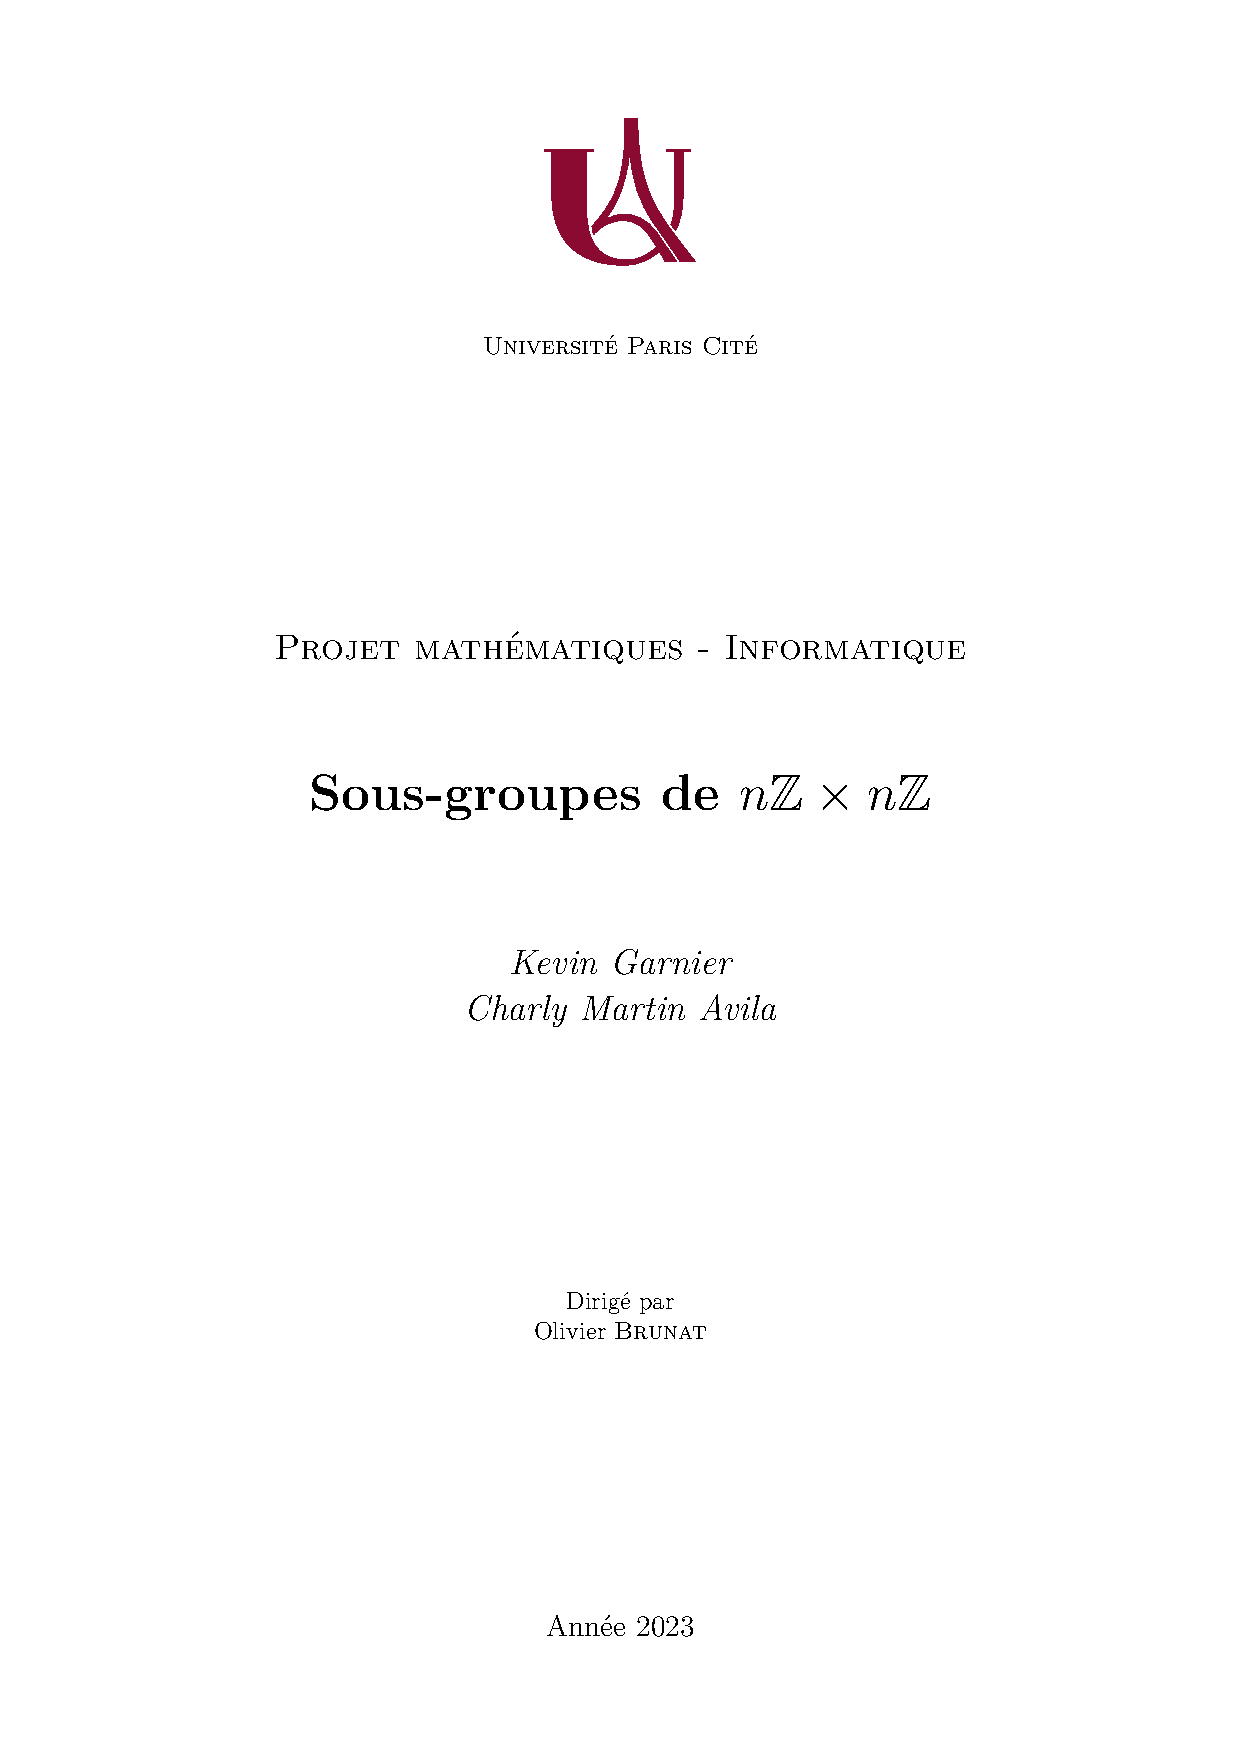
\includepdf{title.pdf}
\tableofcontents
\newpage

\section{Introduction}
	Il est très facile de décrire tous les sous-groupes d'un groupe cyclique
	d'ordre $n$ : il y en a exactement un par diviseur positif de $n$.
	Pourtant, étonnamment, décrire tous les sous-groupes d'un groupe abélien
	est en général un problème difficile.\\
	Dans ce projet, nous nous se proposons de considérer cette question pour le groupe $\ZZ$.

	D'un point de vue théorique, nous mettrons en avant la générations et la caractérisations de \\
	sous-groupes grâce aux vecteurs colonne des matrices à coefficients entier et en particulier aux formes
	normales de Hermite. Nous montrerons aussi une formule permettant de les compter.

	D'un point de vue pratique, nous créerons un programme \textsc{OCaml} capable de générer les\\
	sous-groupes de $\ZZ$ ainsi que leur treillis à partir d'un entier donné en paramètres.
\section{Quelques simplifications du problème}
\subsection{Décomposition de $n$ en éléments irréductibles}
Nous pouvons tout d'abord simplifier le problème aux cas où $n = p^m$ avec $p$ un nombre premier
et $m \in \N$. En effet, soit
$$n = \prod_i^k p_i^{\alpha_i}$$
Par le théorème des restes chinois, on a
$$ \ZnZ \isom (\Z/p_i^{\alpha_i}\Z) \x \cdots \x (\Z/p_i^{\alpha_i}\Z)$$
En particulier,
\begin{equation*}
	\begin{split}
		\ZZ & \isom
		(\Z/p_i^{\alpha_i}\Z) \x \cdots \x (\Z/p_i^{\alpha_i}\Z) \x (\Z/p_i^{\alpha_i}\Z) \x \cdots \x (\Z/p_i^{\alpha_i}\Z)\\
			& \isom (\Z/p_i^{\alpha_i}\Z)^2 \x \cdots \x (\Z/p_i^{\alpha_i}\Z)^2
	\end{split}
\end{equation*}

En pratique, pour décomposer en entier en facteurs irréductibles, nous avons utilisé la procédure de
\textsc{$\rho$-Pollard} pour obtenir un diviseur de $n$:
\begin{verbatim}
fonction rho_pollard P x y k i d
  si d <> 1 Retourne d
  sinon
    x = P(x) mod n
    d = pgcd(|y - x|, n)
    Si i = k
      Alors Retourne rho_pollard loop P x x 2k (i + 1) d
    Sinon Retourne rho_pollard P x y k (i + 1) d
\end{verbatim}
Dans notre implémentation, $P(X) = X^2 - 1$.\\
Puis nous répétons la procédure jusqu'à que les diviseurs soient premier.
En triant et en regroupant les nombres premier, nous obtenons donc les différents $p^{\alpha_i}_i$

\newpage
\subsection{Simplification des sous-groupes}
Soit \app{\varphi}{\Z^2}{\ZZ}{(a,b)}{(\bar a, \bar b)}
$\varphi$ est surjective par définition de la classe d'équivalence de a et b.
Montrons que $\ker \varphi = n\Z \x n\Z$.

\begin{equation*}
	\begin{split}
		&(a,b) \in \ker \varphi \\
		&\text{ssi } \varphi(a,b) = (\bar 0, \bar 0)\\
		&\text{ssi } (\bar a, \bar b) = (\bar 0, \bar 0)\\
		&\text{ssi } \bar a = \bar 0 \text{ et } \bar b = \bar 0\\
		&\text{ssi } a \in n\Z \text{ et } b \in n\Z\\
		&\text{ssi } (a,b) \in  n\Z \x n\Z
	\end{split}
\end{equation*}
Ainsi par le premier théorème d'isomorphisme, on a
$$\Z^2/n\Z \x n\Z \isom \ZZ $$
Ainsi le problème se résout à trouver les sous-groupes $H$ de $\Z^2$ tels que
$Mat \; H = \matsqr{a}{0}{b}{c}$\\
et
$n\Z \x n\Z \subseteq H = \gen{\vectcolsqr{\bar a}{\bar b}, \vectcolsqr{0}{\bar c}}$


\section{Matrices à coefficients entier et forme normales de Hermite}
%problème section précédente, il existe un nombre important de matrice similaire i.e qui
%engendre le même sous groupe
\subsection{Matrices à coefficients entier}
% TODO : ajouter demo en rapport avec les matrice im AQ= im A
\subsection{Forme normale de Hermite}
% preuve existence ?
% algo forme hermite
% preuve AX = C solution ssi on peut annuler C ?

\section {Génération et énumération des sous-groupes}
\subsection{Génération des sous-groupes}
%preuve sur la bonne forme de forme normale de Hermite
\subsection{Énumération des sous-groupes}
%preuve sur le calcul du nombre de sous-groupe

\section{Génération du treillis}
%preuve H C H' <=> Hermite(H'|H) = H'
%Algorithme génération du treillis
%Choix de .dot et graphivz

\section {Quelques résultats}
\subsection{Pour n = 2}
%pour n = 2
\subsection{Pour n = 4}
% pour n = 4
\subsection{Pour n = 20}
% pour n = 20

%nombre de sous-groupes + treillis .dot

\section{Références}
%livre d'algo
%poly du prof

\end{document}
